\chapter{Video Segmentation and Low-Level Features}% }%/Algorithm/Approach/Setup}
\label{chapter3}
In this chapter we aim to analyze the quality of low-level features applied to video segmentation.
In order to study this problem, we first need to choose the video segmentation model, which gives a strong representation
with a variety of motion- and appearance-based features and provides the maximum computational reduction.% and lends a variety of motion- and appearance-based features. 

In our work we propose to use superpixel-based approach of~\cite{GalassoCS12}, as it yields the reduction of computational complexity 
and also defines powerful within- and between-frame affinities, which is the key to producing high-quality video segmentation results with object-level details.
We evaluate the quality of suggested in~\cite{GalassoCS12} low-level features on the Berkeley motion segmentation dataset~\cite{Brox10}.
% and the boundary and volume oriented benchmark metrics~\cite{Galasso13} were chosen.
\section{Video Segmentation Model}%/with Superpixels Approach}
\label{sec:ch3_framework}
In this thesis we follow the same pipeline as in the work of~\cite{GalassoCS12}. The method proposes to over-segment the video as a basis for further processing. Here the two-step approach is employed. 

The first step is pixel-based and results in a motion-aware hierarchical image segmentation (MAHIS). The affinities
are calculated from brightness, color and texture gradients as in the previous work of~\cite{Arbelaez09}, plus the additional cue - the flow gradient - is considered. Adding the motion cue allows to overcome some problems, when
appearance features are not discriminative enough, and therefore to detect better boundaries. 
Then in the same setup as~\cite{Arbelaez11} all the features 
are passed by the contour detector to the graph construction and partitioning via the spectral clustering, and after that the OWT-UCM machinery is applied to produce hierarchical image segmentation. From the finest obtained 
oversegmentation we extract superpixels. 

The second step is superpixel-based and uses different types of similarities inside a single frame and across multiple frames. Considering the between-frame similarity measures enables temporal consistency of segments and hence leads
to better video segmentation results.
Employing superpixels provides a significant computational reduction, since the number of elements is lessened by several orders of magnitude, and allows more powerful representation of 
within- and between-frame affinity measures (see sec.~\ref{sec:ch3_affinities}).

Next the affinity matrix $W$ is formed based on pair-wise similarity scores $w_{ij}$ between superpixels $i$ and $j$. The weight $w_{ij}$ is calculated as a normalized product of the similarity measures listed below
(sec.~\ref{sec:ch3_affinities}). The resulted matrix $W$ is sparse since only spatial and temporal neighbourhood is considered, which makes the computational process feasible. The matrix $W$ is quadratic in the number of elements
and superpixels are ordered according to their top-down left-right position in their frame and to their frame.

After constructing the similarity matrix to obtain the final segmentation we consider clustering as a graph partitioning problem and employ different spectral relaxation techniques (see sec.~\ref{SpectRelax}).
We chose spectral clustering framework due to its well-understood mathematical background, recent advances in graph partitioning and also state-of-art performance in a number of areas including image~\cite{Shi00,Arbelaez11} 
and video object segmentation~\cite{Brox10,GalassoCS12,Galasso14}.  

Therefore the overall performance of the proposed video segmentation method highly depends on three main aspects:
\begin{itemize}
\item defined within- and between-frame affinities;
\item structure of similarity graph;
\item choice of spectral clustering method and graph cut objective function.
\end{itemize}

The outline of the video segmentation model is listed in Algorithm~\ref{alg::VSM}. 
\incmargin{1em} 
\begin{algorithm}[htbp]
\caption{Video Segmentation Method}
\label{alg::VSM}
\dontprintsemicolon
\BlankLine
\Indm  
\Setnlsty{textbf}{}{:}
\Indp
\BlankLine
extract superpixels from the lowest hierarchical level of pixel-based segmentation, obtained via MAHIS;\\
compute low-level video features based on superpixels;\\ 
construct a graph with an affinity matrix formed of pair-wise within- and between-frame similarity measures;\\
apply spectral clustering technique for partitioning of the constructed graph to obtain final video segmentation.
\BlankLine
\Indm  
\end{algorithm}
\decmargin{1em}
% \incmargin{1em} 
% \begin{algorithm}[htbp]
% \caption{Video Segmentation Method}
% \label{alg::VSM}
% \dontprintsemicolon
% \BlankLine
% \Indm  
% \Setnlsty{textbf}{}{:}
% \Indp
% \BlankLine
% do pixel-based segmentation via MAHIS;\\
% generate Ultrametric Contour Maps (UCM);\\
% extract superpixels from the lowest hierarchical level of the UCM;\\
% construct affinity matrix based on within- and between-frame similarity measures;\\
% %learn must-link constraints using within- and between-frame affinities as features;\\
% %construct the reduced graph by integrating must-link constraints via sparsification;\\
% apply spectral relaxation technique to obtain final video segmentation.
% \BlankLine
% \Indm  
% \end{algorithm}
% \decmargin{1em}

\begin{figure}[t]
\centering
\subfigure[Video Sequence]{%
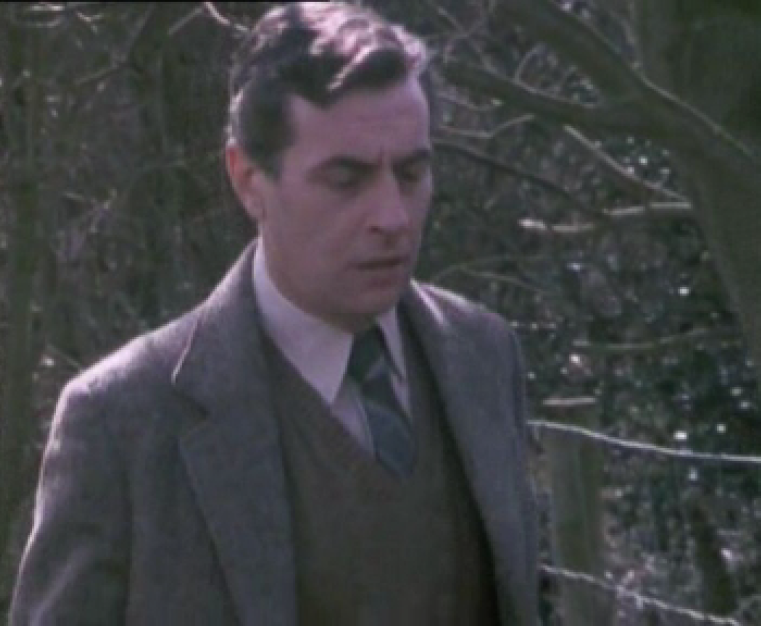
\includegraphics[width=0.185\textwidth]{images/png/pipe_1.png}
\label{fig:subfigure1}}
%\quad
\subfigure[Ultrametric Contour Map (UCM)]{%
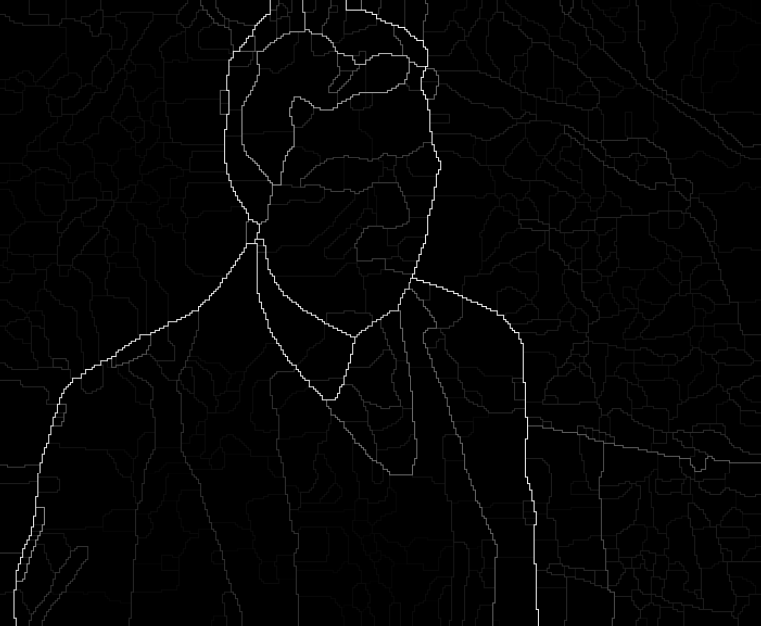
\includegraphics[width=0.185\textwidth]{images/png/pipe_5.png}
\label{fig:subfigure2}}
%\quad
\subfigure[Superpixels]{%
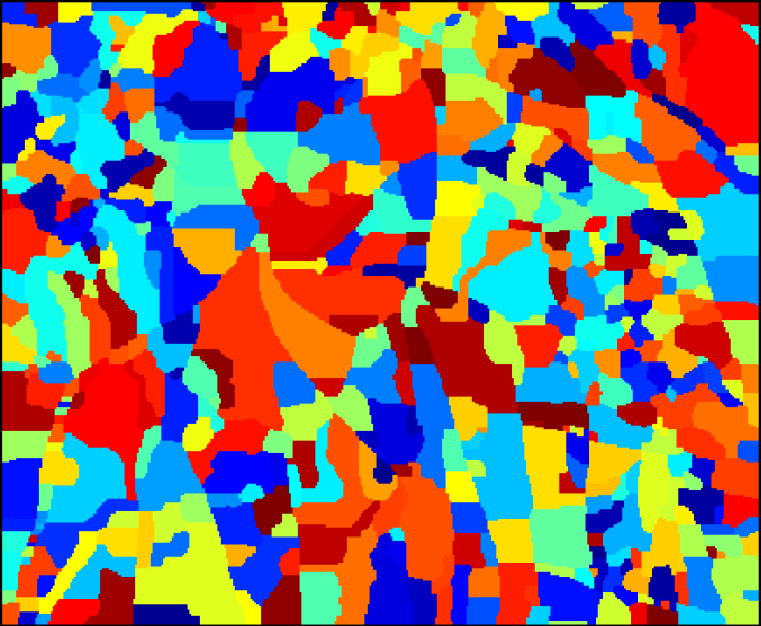
\includegraphics[width=0.185\textwidth]{images/png/pipe_2.png}
\label{fig:subfigure1}}
%\quad
\subfigure[Affinity Matrix]{%
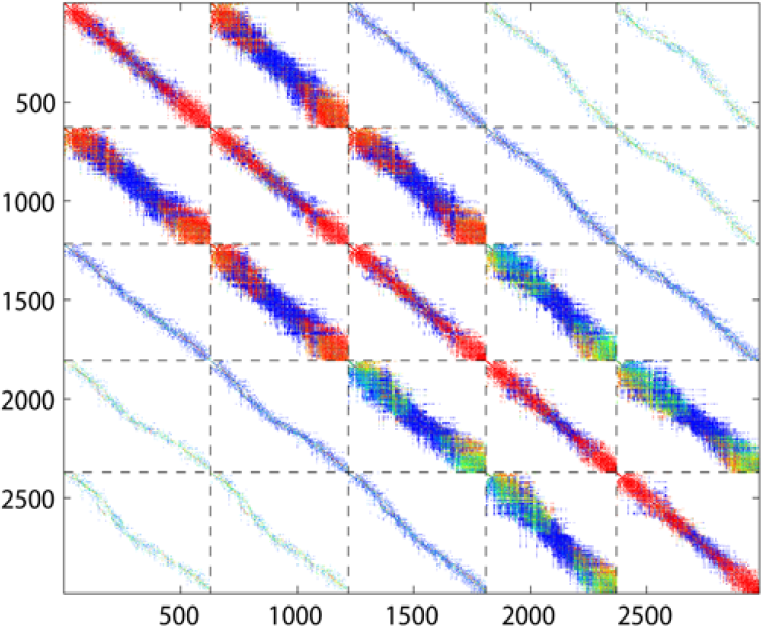
\includegraphics[width=0.185\textwidth]{images/png/pipe_3.png}
\label{fig:subfigure2}}
%\quad
\subfigure[Segmentation]{%
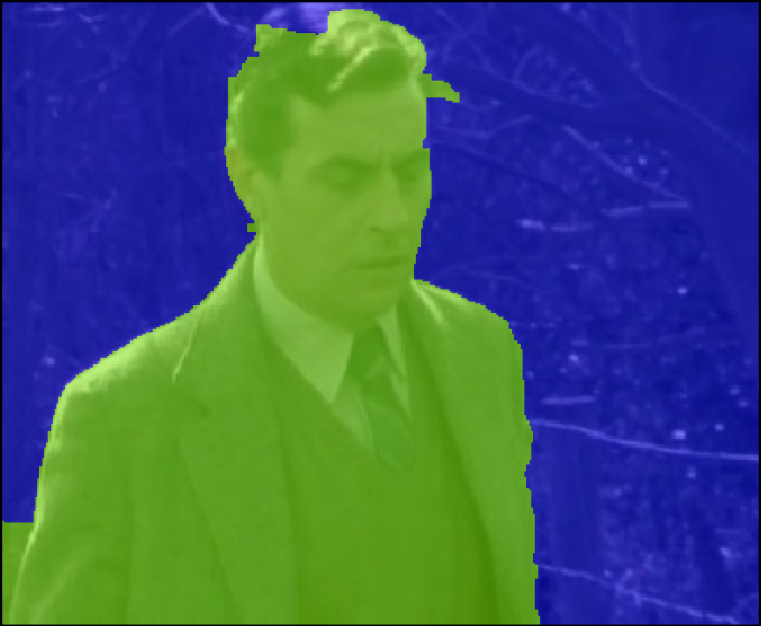
\includegraphics[width=0.185\textwidth]{images/png/pipe_4.png}
\label{fig:subfigure2}}
%\quad
\caption[Video segmentation pipeline]{
{\bf Video segmentation pipeline} (courtesy of~\cite{GalassoCS12}).} % We generate Ultrametric Contour Maps (UCM) via MAHIS, extract superpixels from the lowest hierarchical level of UCM, 
%construct affinity matrix based on within- and between-frame similarity measures,
%and apply spectral relaxation technique to obtain final video segmentation.}
\label{fig:seg_example}
\end{figure}
The source code of the work~\cite{GalassoCS12} can be found at \url{http://www.mpi-inf.mpg.de/~galasso/files/VSS.zip}.
\section{Superpixel Affinities for Video Segmentation}
\label{sec:ch3_affinities}
%After extracting superpixels, to derive the final video segmentation result we need to compute superpixel affinity measures. 
In a graph-theoretic approach, the overall segmentation quality highly depends on the graph affinities. Therefore, to produce high-quality segmentation results with object-level details, 
it is important to define the graph affinities gained by integrating local grouping cues.

Following~\cite{GalassoCS12} in this work we employ and analyze low-level features, which are grouped into three categories:
within-frame, between-frame and combined between- and within-frame affinities. Intuitively, using information not only within a single frame, but across multiple frames should lead to better video segmentation performance.
The superpixel-based affinities are calculated from raw features, such as brightness, color, as well as optical flow.
\subsection{Within-Frame Affinities}
The first two affinity terms measure the similarity near the common boundary between superpixels.
\subsubsection*{Across Boundary Appearance (ABA)}
The appearance based term directly uses the ultrametric contour maps of the MAHIS algorithm. The affinity $w^{aba}$ between superpixels $p_f^i$ and $p_f^j$ is defined as the average value $\overline{v}_f^{ij}$ of the contour map along
the common boundary:
\begin{equation*}
 w^{aba}_{p_f^i,p_f^j} = \overline{v}_f^{ij}.
\end{equation*}
\subsubsection*{Across Boundary Motion (ABM)}
The motion based term measures the similarity of the median motion along the common boundary of two superpixels. Given the spatially and temporally ($\pm2$ frames) median filtered optical flow $\overline{u}^f(x)$ and the set of pixel
pairs on opposite side of the common boundary $\psi_f^{ij}$, the ABM score $w^{abm}$ is defined as:
\begin{equation*}
 w^{abm}_{p_f^i,p_f^j} = \exp {\Biggl \{ -\lambda_{abm} \frac{ \sum_{(x_i^m,x_j^m) \in \psi_f^{ij}} \lVert \overline{u}^f(x_i^m) - \overline{u}^f(x_j^m) \rVert^2}{\lvert \psi_f^{ij} \rvert} \Biggr\}}.
\end{equation*}   
\subsection{Between-Frame Affinities}
The affinity terms defined here measure the spatial overlap of pixels in different frames. While the STT allows to calculate similarities between superpixels in neighbouring frames ($\pm2$ frames), the LTT can measure
affinities that might be hundreds of frames apart due to the long-term point trajectories.
\subsubsection*{Short Term Temporal (STT)}
Given superpixel $p_f^i$ at frame $f$ with binary support mask $m_{p_f^i}$ and superpixel $p_{f'}^j$ at frame $f' = f\pm1,2$ with mask $m_{p_{f'}^j}$, the STT affinity measures their overlap with the Dice coefficient by propagating the
 binary mask of superpixel $p_f^i$ with optical flow to the neighbouring frame $f'$:
\begin{equation*}
  w^{stt}_{p_f^i,p_{f'}^j}=\frac{2 \bigr \rvert m^{f'}_{p_f^i} \bigcap m_{p_{f'}^j} \bigl \lvert}{\bigr \rvert m^{f'}_{p_f^i}  \bigl \lvert+ \bigr \rvert m_{p_{f'}^j}  \bigl \lvert}.
\end{equation*}
\subsubsection*{Long Term Temporal (LTT)}
This overlap term is built on long-term point-trajectories. Let $\varPhi_{p_f^i}$ be the subset of trajectories intersecting superpixel $p_f^i$. The LTT affinity score between superpixels $p_f^i$ and $p_{f'}^j$,
$f' = f+N$, $N\neq 0$ is defined as the Dice measure between intersection sets $\varPhi_{p_f^i}$ and $\varPhi_{p_{f'}^j}$ of superpixels:
\begin{equation*}
  w^{ltt}_{p_f^i,p_{f'}^j}=\frac{2 \bigr \rvert \varPhi_{p_f^i} \bigcap \varPhi_{p_{f'}^j} \bigl \lvert}{\bigr \rvert\varPhi_{p_f^i}\bigl \lvert+ \bigr \rvert \varPhi_{p_{f'}^j} \bigl \lvert}.
\end{equation*}
\begin{figure}[t!]
 \centering
 \subfigure[ABM]{%
 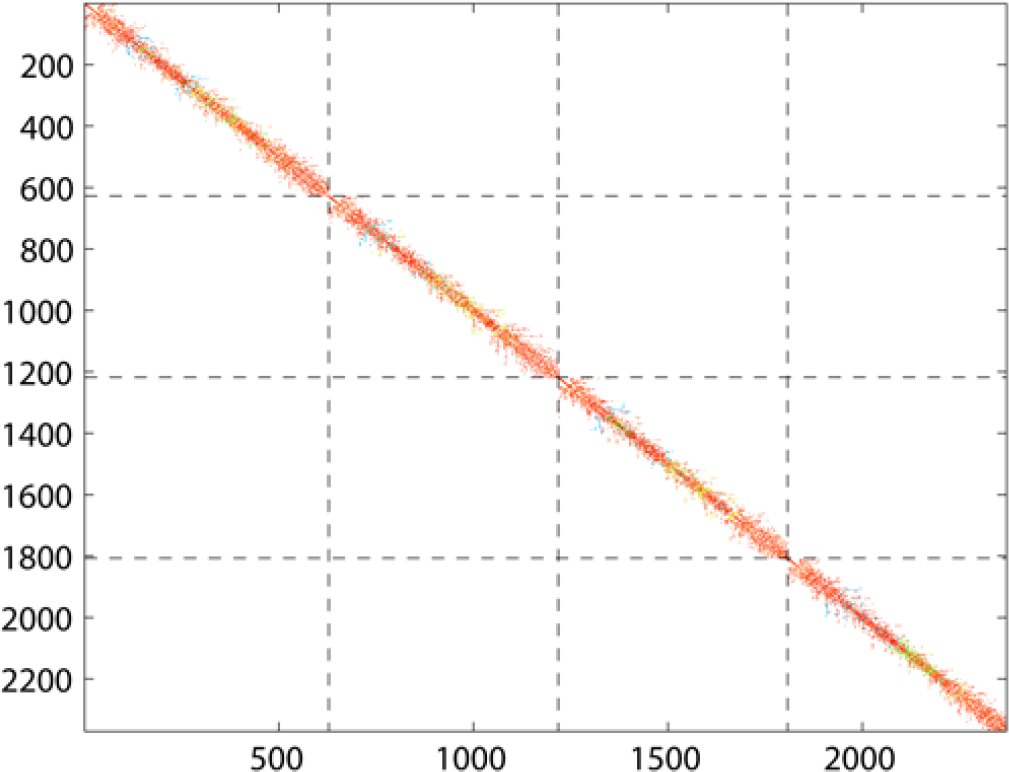
\includegraphics[width=0.2\textwidth]{images/png/abm.png}
\label{fig:subfigure1}}
\quad
 \subfigure[STT]{%
 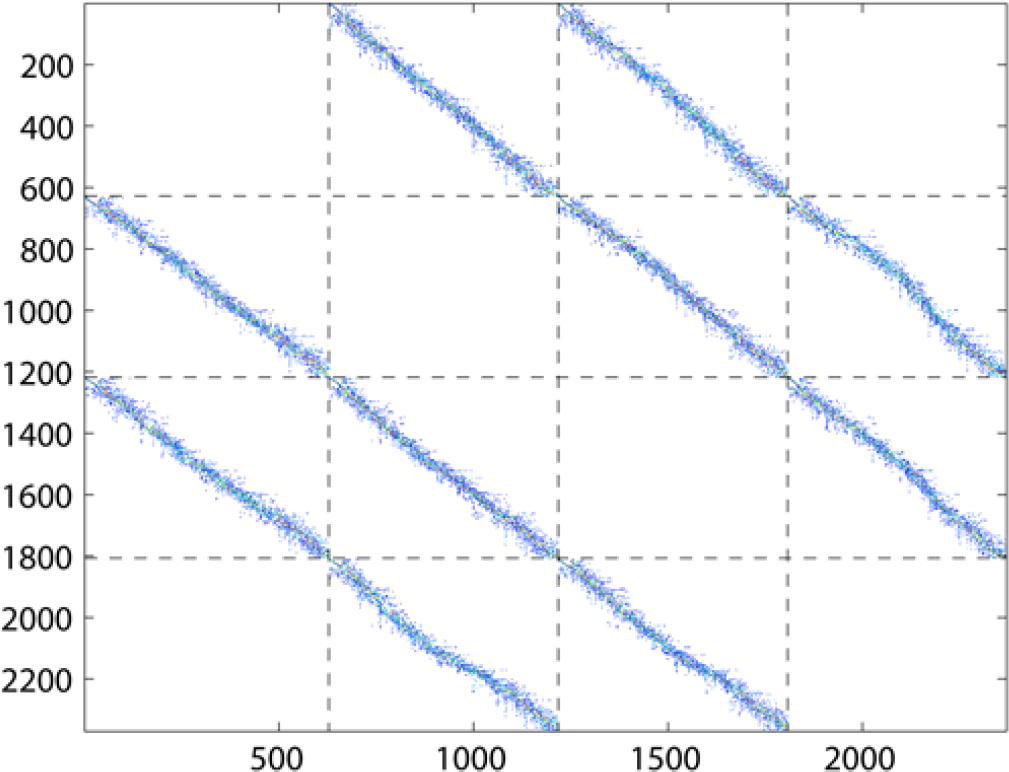
\includegraphics[width=0.2\textwidth]{images/png/stt.png}
\label{fig:subfigure2}}
\quad
\subfigure[LTT]{%
 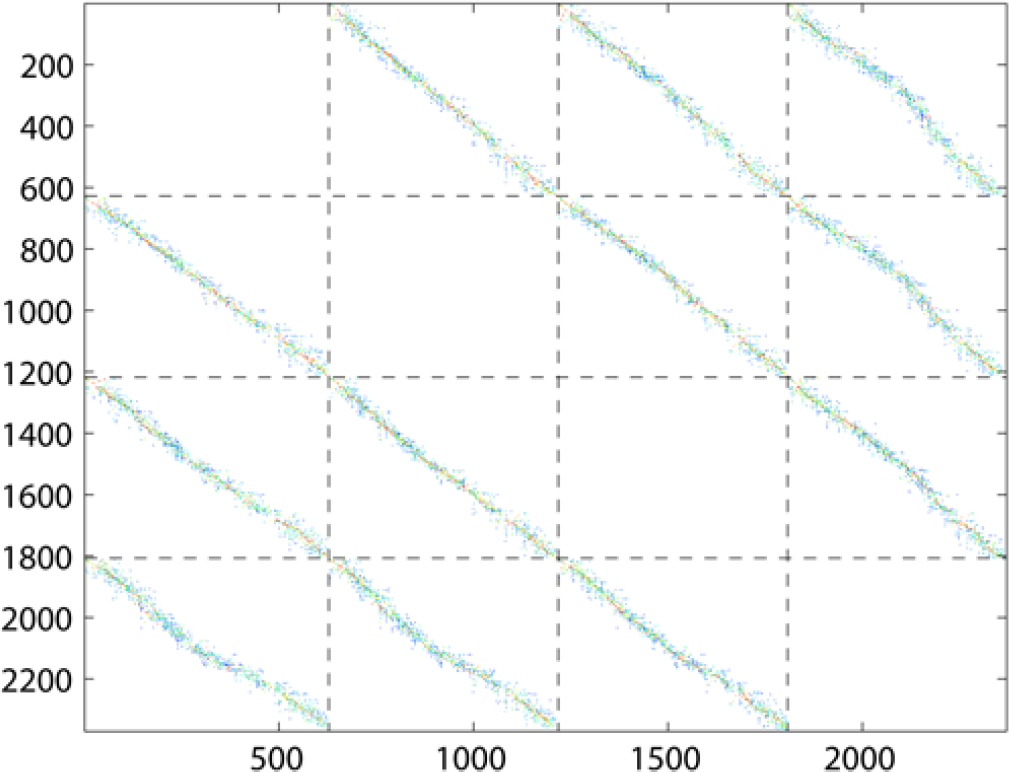
\includegraphics[width=0.2\textwidth]{images/png/ltt.png}
\label{fig:subfigure1}}
\quad
 \subfigure[STM]{%
 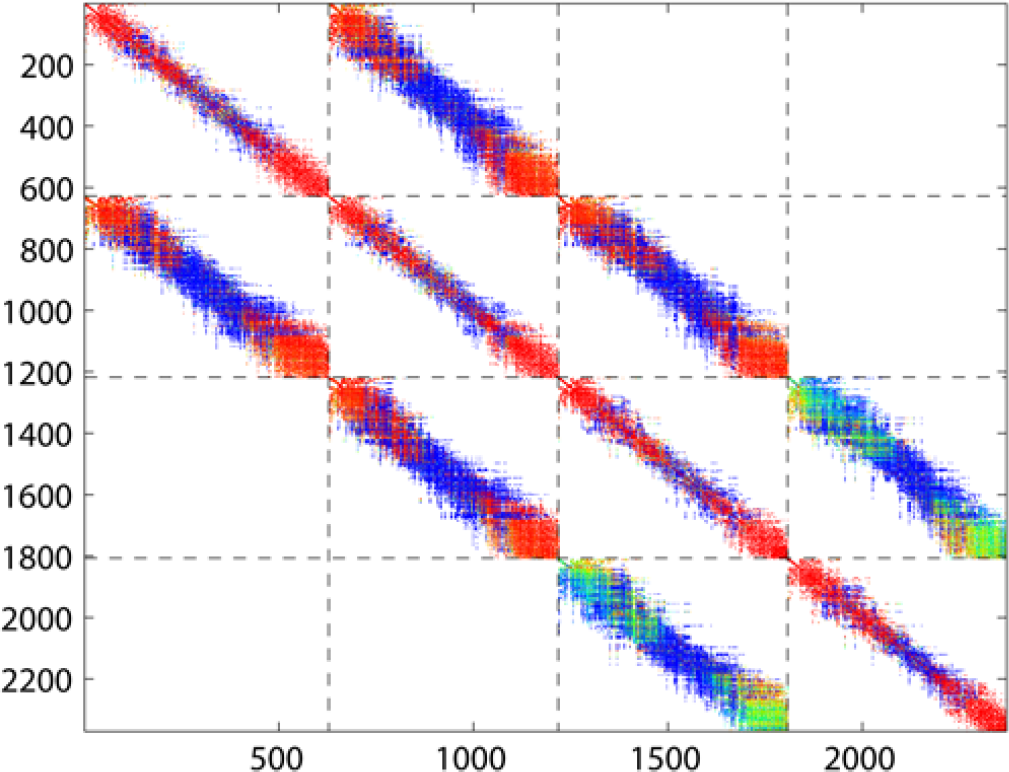
\includegraphics[width=0.2\textwidth]{images/png/stm.png}
\label{fig:subfigure2}}
 \caption[Structure and sparsity of the affinity matrices]{
  {\bf Structure and sparsity of the affinity matrices} (courtesy of~\cite{GalassoCS12}). Terms on the diagonal correspond to within-frame affinities and off the diagonal to between-frame affinities.}
\label{fig:seg_example}
\end{figure}
\subsection{Within- and Between-Frame Affinities}
This group of affinities measures similarities between superpixels in a spatio-temporal neighbourhood ($\pm1$ frame) based on motion and appearance. 
\subsubsection*{Spatio-Temporal Appearance (STA)}
To calculate the appearance term the median brightness and color of a superpixel in CIE Lab color space are used. The STA affinity between superpixels $p_f^i$ and $p_{f'}^j$
is denoted as:
\begin{equation*}
w^{sta}_{p_f^i,p_{f'}^j} = \exp {\bigl \{ -\lambda_{sta} \lVert \overline{Lab}_{p_f^i} - \overline{Lab}_{p_{f'}^j} \rVert \bigr\}}.
\end{equation*}
\subsubsection*{Spatio-Temporal Motion (STM)}
This affinity focuses on motion to allow grouping of superpixels of the same moving objects, based on the median optical flow $\overline{u}_{p_f^i}$ of the superpixel $p_f^i$.
The STM term is defined as:
\begin{equation*}
w^{stm}_{p_f^i,p_{f'}^j} = \exp {\bigl \{ -\lambda_{stm} \lVert \overline{u}_{p_f^i} - \overline{u}_{p_{f'}^j} \rVert^2 \bigr\}}.
\end{equation*}

It has been shown in~\cite{GalassoCS12}, that the set of affinities STT+LTT+STM+STA gives the same qualitative result as the combination of all of them. The temporal terms STT and LTT quite successfully track objects, but suffer from 
``jittering'' effect, caused by the lack of the precision of optical flow and large motion. The spatio-temporal affinities STM and STA become more effective when the strong motion and color differences occur between clusters.
STT+LTT and STM are complementary motion terms supplemented by STA.
\section{The Berkeley Motion Segmentation Dataset}% Evaluation and Dataset
\label{sec:ch3_dataset}
In order to evaluate the results we need to choose a dataset, which should contain diverse video sequences with a variety of objects and different kinds of motion. Plus it should offer a dense ground truth annotation.
There exist a large number of various datasets for video segmentation, but the majority of them are limited in aforementioned aspects. CamVid~\cite{BrostowFC09} includes only a few sequences, as well as~\cite{Grundmann10,XuCorso12}. 
In Figment~\cite{FragkiadakiZS12} all the objects are of the same size. The Hopkins 155 dataset~\cite{TronV07} has many video sequences, but ground truth is only available for a very sparse set of points.
The dataset of~\cite{Galasso13} has multiple human annotations and fulfills the criteria of diversity, but the sequences are of HD quality, which is computationally expensive. 

Therefore we decided to evaluate all the results on the Berkeley motion segmentation dataset (BMDS), which was provided by~\cite{Brox10}. The dataset consists of 26 video sequences of varying length with a pixel-accurate segmentation annotation of 
moving objects, with a total of 189 annotated frames. The annotation is dense in space and sparse in time, with more frames being annotated at the beginning of a shot. The ground truth segmentation
mask is provided roughly for every 10th frame.
\begin{figure}[h]
 \centering
 \subfigure{%
 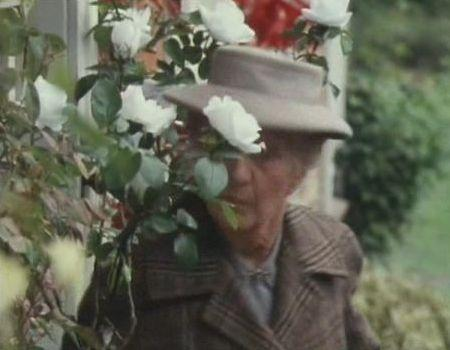
\includegraphics[width=0.13\textwidth]{images/png/M7/marple7_001.jpg}}
\subfigure{%
 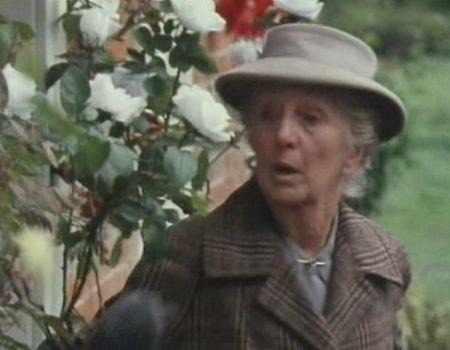
\includegraphics[width=0.13\textwidth]{images/png/M7/marple7_010.jpg}}
\subfigure{%
 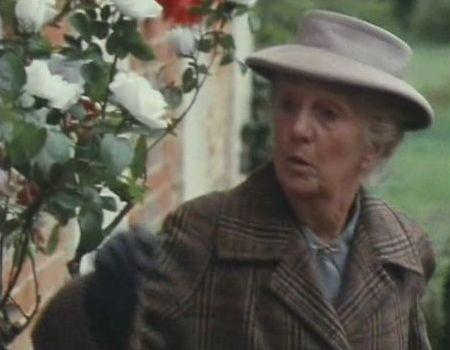
\includegraphics[width=0.13\textwidth]{images/png/M7/marple7_020.jpg}}
\subfigure{%
 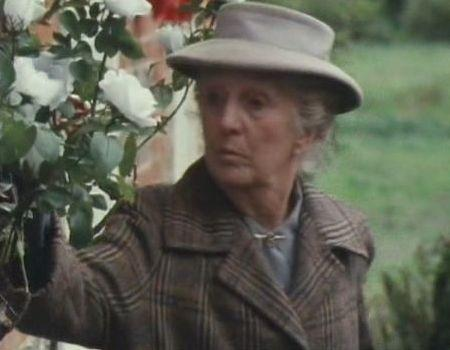
\includegraphics[width=0.13\textwidth]{images/png/M7/marple7_030.jpg}}
\subfigure{%
 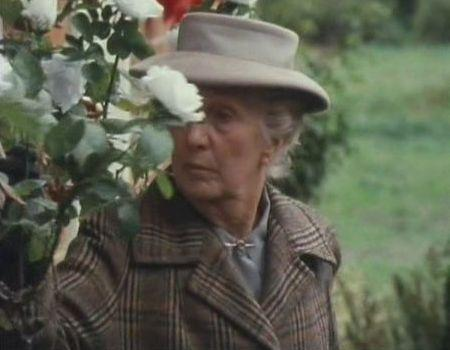
\includegraphics[width=0.13\textwidth]{images/png/M7/marple7_040.jpg}}
\subfigure{%
 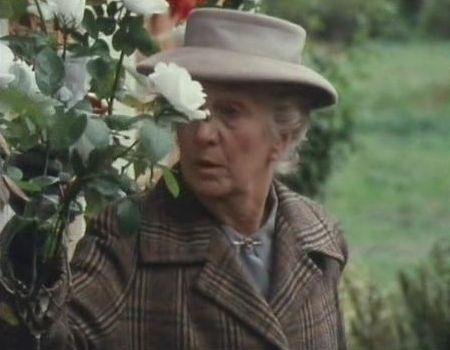
\includegraphics[width=0.13\textwidth]{images/png/M7/marple7_050.jpg}}
\subfigure{%
 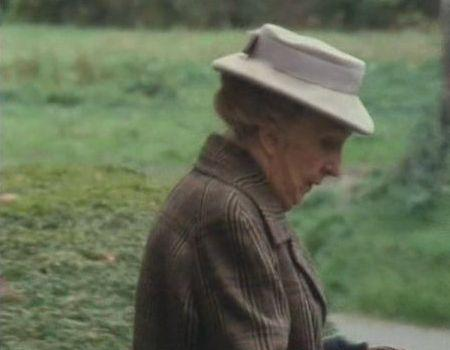
\includegraphics[width=0.13\textwidth]{images/png/M7/marple7_100.jpg}}

 \subfigure{%
 
\includegraphics[width=0.13\textwidth]{images/png/M7/marple7_001.png}}
\subfigure{%
 
\includegraphics[width=0.13\textwidth]{images/png/M7/marple7_010.png}}
\subfigure{%
 
\includegraphics[width=0.13\textwidth]{images/png/M7/marple7_020.png}}
\setcounter{subfigure}{0}
\subfigure[Marple7]{%
 
\includegraphics[width=0.13\textwidth]{images/png/M7/marple7_030.png}}
\subfigure{%
 
\includegraphics[width=0.13\textwidth]{images/png/M7/marple7_040.png}}
\subfigure{%
 
\includegraphics[width=0.13\textwidth]{images/png/M7/marple7_050.png}}
\subfigure{%
 
\includegraphics[width=0.13\textwidth]{images/png/M7/marple7_100.png}}

%  \caption[Video sequence ``Marple7'' from the BMDS and its annotated ground truth]{
%   {\bf Video sequence ``Marple7'' from the BMDS and its annotated ground truth}.}
% \label{fig:seg_example}
% \end{figure}
% 
% \begin{figure}[h!]
%  \centering
 \subfigure{%
 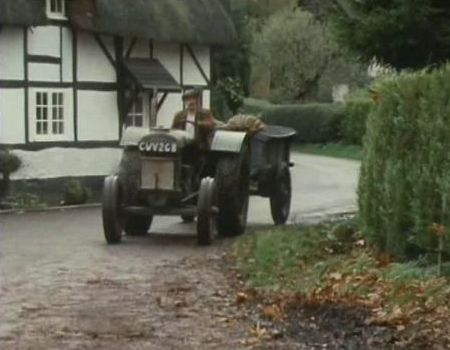
\includegraphics[width=0.13\textwidth]{images/png/M8/marple8_01.jpg}}
\subfigure{%
 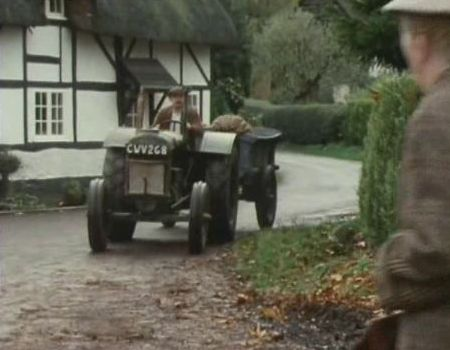
\includegraphics[width=0.13\textwidth]{images/png/M8/marple8_10.jpg}}
\subfigure{%
 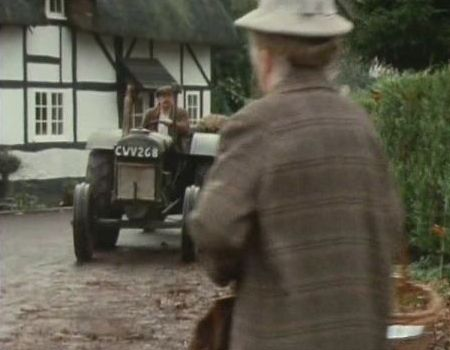
\includegraphics[width=0.13\textwidth]{images/png/M8/marple8_20.jpg}}
\subfigure{%
 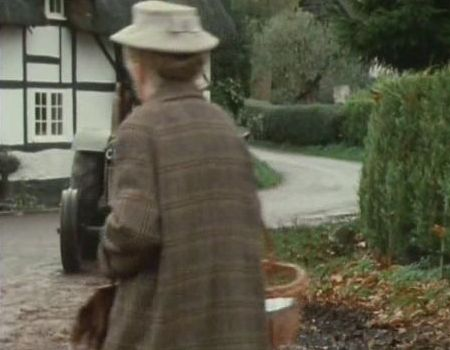
\includegraphics[width=0.13\textwidth]{images/png/M8/marple8_30.jpg}}
\subfigure{%
 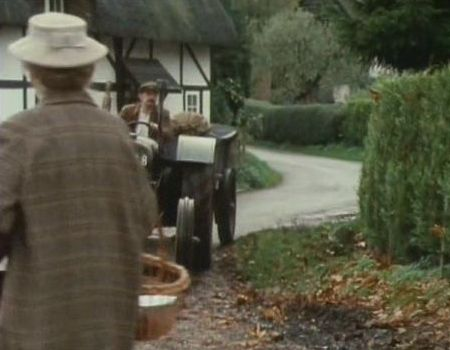
\includegraphics[width=0.13\textwidth]{images/png/M8/marple8_40.jpg}}
\subfigure{%
 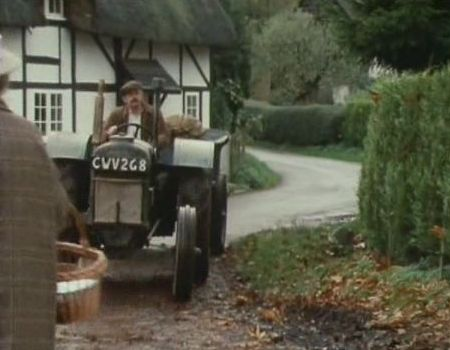
\includegraphics[width=0.13\textwidth]{images/png/M8/marple8_50.jpg}}
\subfigure{%
 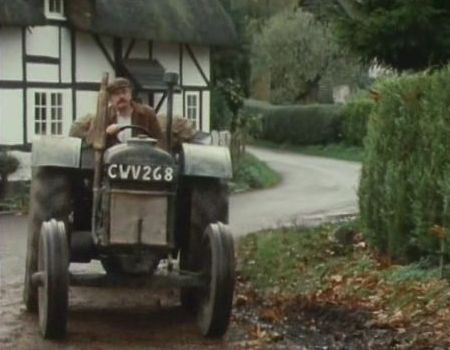
\includegraphics[width=0.13\textwidth]{images/png/M8/marple8_72.jpg}}

 \subfigure{%
 
\includegraphics[width=0.13\textwidth]{images/png/M8/marple8_01.png}}
\subfigure{%
 
\includegraphics[width=0.13\textwidth]{images/png/M8/marple8_10.png}}
\subfigure{%
 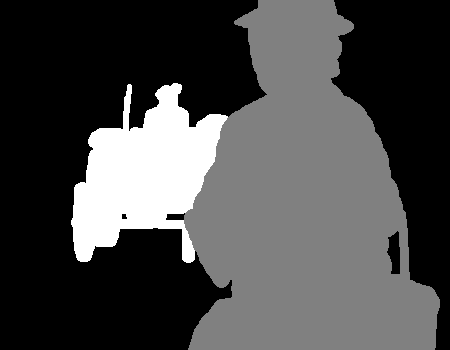
\includegraphics[width=0.13\textwidth]{images/png/M8/marple8_20.png}}
\setcounter{subfigure}{1}
\subfigure[Marple8]{%
 
\includegraphics[width=0.13\textwidth]{images/png/M8/marple8_30.png}}
\subfigure{%
 
\includegraphics[width=0.13\textwidth]{images/png/M8/marple8_40.png}}
\subfigure{%
 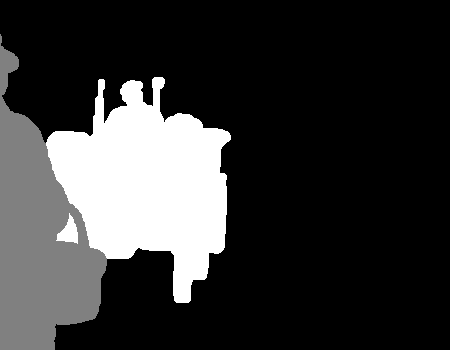
\includegraphics[width=0.13\textwidth]{images/png/M8/marple8_50.png}}
\subfigure{%
 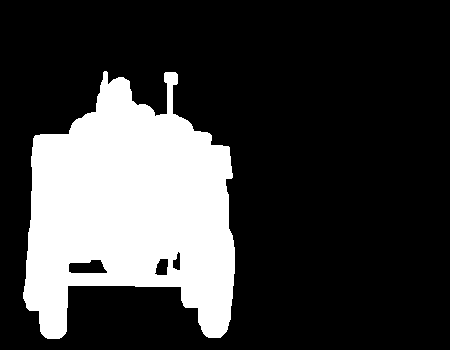
\includegraphics[width=0.13\textwidth]{images/png/M8/marple8_72.png}}

 \caption[Examples of video sequences from the BMDS and its annotated ground truth]{
  {\bf Examples of video sequences from the BMDS and its annotated ground truth}.}
\label{fig:seg_example}
\end{figure}

The dataset includes people, cars and other objects, and various degrees of motion, including camera and object motion. All the sequences are of VGA quality.
The BMDS contains 10 sequences of outdoor traffic taken with a handheld camera and two sequences of people in movement, taken from the Hopkins 155 dataset, and 13 sequences from the TV series ``Miss Marple''. 
% A total of 
% 189 frames is annotated. 12 of the sequences, 10 car and 2 people sequences, are taken from the Hopkins 155 dataset. 

In order to focus the challenge more on segmentation, rather than interest point detection or tracking, the sets of tracked interest points for every video are provided. The dataset also comes with evaluation 
benchmark~\cite{Galasso13} that allows direct comparison of results. 

We decided to use the BMDS because it captures real-life situations, has a reasonable complexity and is also challenging for the current video segmentation algorithms as all the sequences exhibit multi-layered
motion. Besides, various papers show results for this dataset and therefore it is good for comparison and evaluation.

For this dataset we provided additional annotation for every 2nd, 9th, and 11th frame with the purpose of evaluation and analysis of behaviour of affinity measures across 1 and 2 frames. 
So now there are 267 ground truth frames in total.
For all the experiments we restricted ourselves to 30 frames.

The dataset and evaluation software can be found at \url{http://lmb.informatik.uni-freiburg.de/resources/datasets/moseg_dataset.zip}.
\section{Analysis of Low-Level Features for Video Segmentation}
\label{sec:ch3_aff}
Little attention has been paid in literature to the features which should be used for video processing.
The purpose of the next group of experiments, described in this section, is to examine the quality of low-level features presented in Section~\ref{sec:ch3_affinities} for the task of video segmentation.
Here we evaluated on all sequences from the BMDS. Particularly we were interested in the annotated frames as we needed to determine true and false connections between superpixels.

We conducted several experiments where the features were tested on the ground truth frames in the same manner. We started with the evaluation of the affinities between non-adjacent annotated frames as 
in the dataset roughly every 10th frame is annotated, on the whole 4 frames for each sequence.
However, the behaviour of the between-frame affinities could be influenced by the temporal neighbourhood. Therefore, to properly evaluate low-level video features the same study was
conducted on the superpixels affinities between 3 adjacent frames. As the BMDS does not have the ground truth for the neighbouring frames, in order to experiment
additionally every 9th and 11th frame was annotated.
\subsection{Evaluation of Superpixels Affinities Between Non-Adjacent Video Frames}
With this group of experiments we aim to examine superpixels affinities based on 4 annotated frames.
The non-negative similarity score between superpixels is set to be true if the superpixels belong to the same object according to the ground truth, otherwise we consider the affinity false.  
The range of affinity varies from 0 to 1.

Figure~\ref{fig:affin_10th} shows the histogram for the superpixel affinities LTT, ABA, ABM, STA, STM, the combined similarity score W and the final weight without the long-term-temporal 
affinity W-LTT. The x-axis represents different affinity measures, the y-axis the range of similarity scores and the z-axis the number of true or false connections in the logarithmic scale.

The STT affinity is not included because it measures the similarity between superpixels across 2 frames and therefore could not be evaluated as we have only every 10th frame annotated.
For the same reason STM and STA are examined only for within-frame connections and LTT for superpixels across more than 10 frames.
\begin{figure}[htbp]
\centering
\addtolength{\subfigcapskip}{0.07in}
\subfigure[True Positives]{%
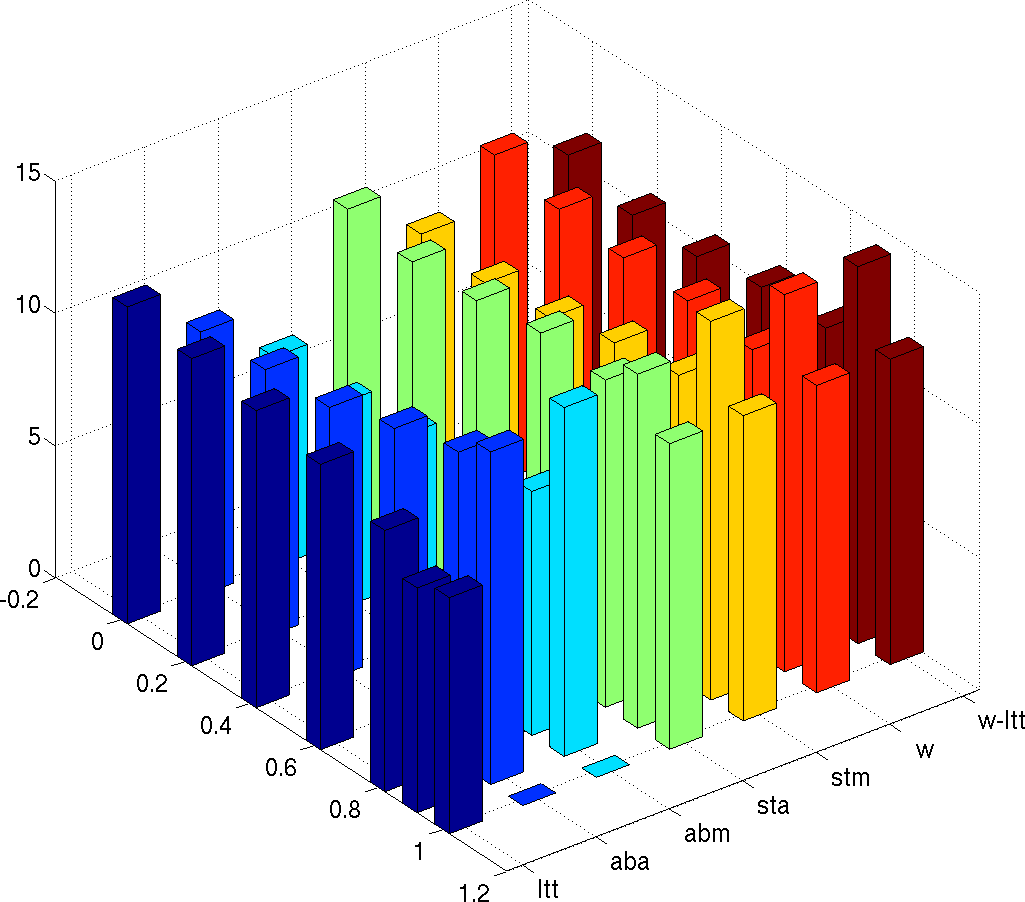
\includegraphics[width=0.45\textwidth]{images/hist/all_old_pos.png}}
\quad%\hfill
% \subfigure{%
% 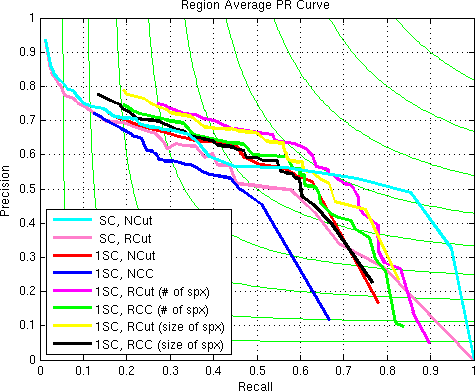
\includegraphics[trim=0cm 0cm 0cm 0.8cm, clip=true, width=0.47\textwidth]{images/basic/3.png}}
\subfigure[False Positives]{%
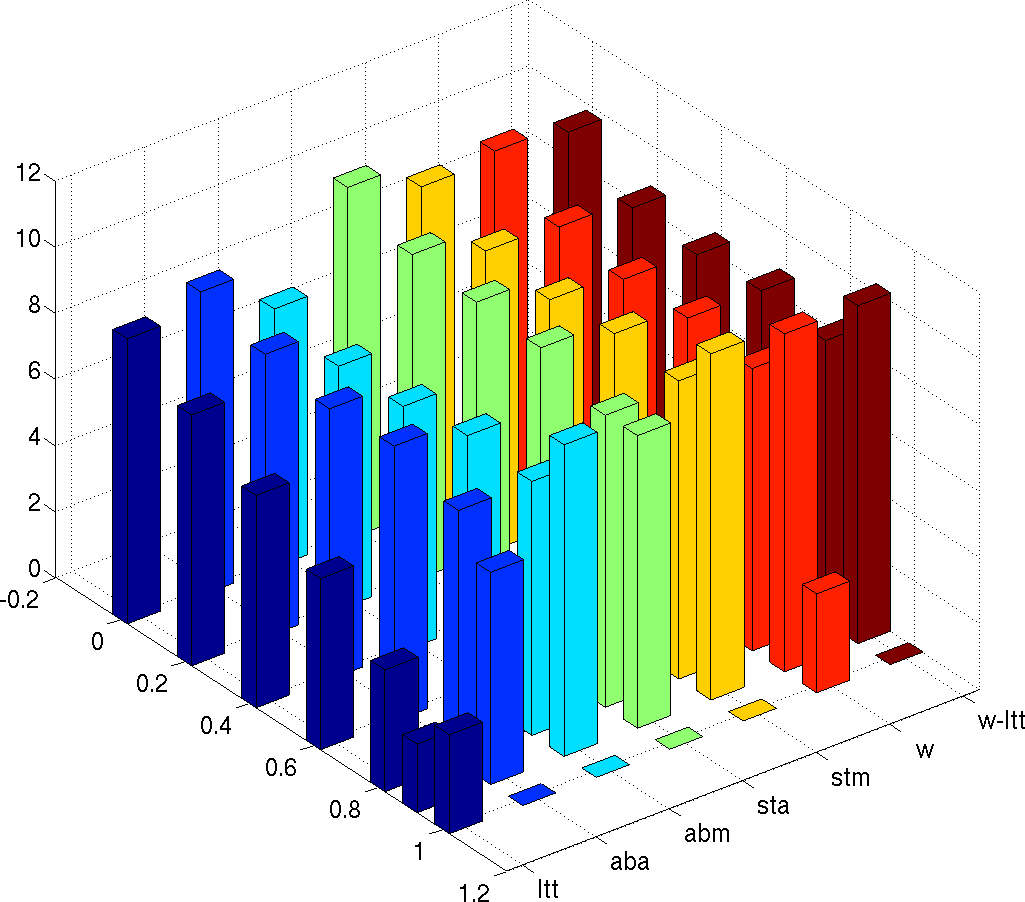
\includegraphics[width=0.45\textwidth]{images/hist/all_old_neg.png}}
\subfigure[Error Rate: $\mathrm{|FP|/|FP+TP|}$]{%
\centering
\scriptsize 
\renewcommand{\arraystretch}{1.3}
\begin{tabular}{|l|@{ }c@{ }|@{ }c@{ }|@{ }c@{ }|@{ }c@{ }|@{ }c@{ }|@{ }c@{ }|@{ }c@{ }|}
\hline
&\textbf{ltt}&\textbf{aba}&\textbf{abm}&\textbf{sta}&\textbf{stm}&\textbf{w}&\textbf{w-ltt}\\\hline
\textbf{0-0.2}&0.0336&0.3132&0.4649&0.1371&0.3388&0.0859&0.1719\\\hline
\textbf{0.2-0.4}&0.0175&0.1732&0.4007&0.1003&0.2564&0.0509&0.1294\\\hline
\textbf{0.4-0.6}&0.0081&0.1089&0.3235&0.0767&0.1765&0.0479&0.1113\\\hline
\textbf{0.6-0.8}&0.0036&0.0599&0.2711&0.0491&0.1249&0.0547&0.0893\\\hline
\textbf{0.8-0.9}&0.0021&0.0161&0.1763&0.0281&0.0781&0.0549&0.0689\\\hline
\textbf{0.9-0.99}&\textbf{0.0016}&\textbf{0.0021}&0.0226&0.0106&0.0209&0.0173&0.0174\\\hline
\textbf{1}&\textbf{0.0026}&-&-&\textbf{0}&\textbf{0}&0.0002&0\\\hline 
\end{tabular}
}
\caption[Evaluation of the LTT, ABA, ABM, STA, STM, W, W-LTT affinities on 4 annotated frames for each video sequence]{
{\bf Evaluation of the LTT, ABA, ABM, STA, STM, W, W-LTT affinities on 4 annotated frames for each video sequence (roughly 1st, 10th, 20th, 30th frame).}}
\label{fig:affin_10th}
\end{figure}

We can see from the histograms that the features perform quite good and only a few mistakes are made for high values of affinities. STA and STM measures equal 1 have zero error rate and for LTT bigger than 0.9 
almost no mistake occurs. This is not surprising, as from the work~\cite{GalassoCS12} we know that LTT and STM affinities are the most contributory to the performance, as well as the STA.

It was observed that the within-frame measure of similarity ABA also has good results, for scores higher than 0.9 the error rate is less than 0.2\%. In the previous work it was mentioned that taking out the boundary
affinity ABA did not alter the performance, although the assessment of the similarity measure shows otherwise. One could assume the reason for this may lie in how the affinities were combined together for the final score.
ABA might be outweighed by other similarity measures. 
LTT shows good performance but still some mistakes occur.
This affinity score is calculated as the ratio of common point trajectories between two superpixels to the average number of trajectories for these superpixels. Therefore it is easier to achieve
higher values for the superpixels which have only a few intersecting trajectories. 

Figure~\ref{fig:ltt_10th} illustrates more detailed examination of LTT. 
Here the x-axis of the histogram represents the number of common trajectories and the y-axis the range of LTT scores. As it can be seen we can avoid a majority of the errors if we restrict
the number of common trajectories to be higher or equal 5.
\begin{figure}[htbp]
\centering
\addtolength{\subfigcapskip}{0.07in}
\subfigure[True Positives]{%
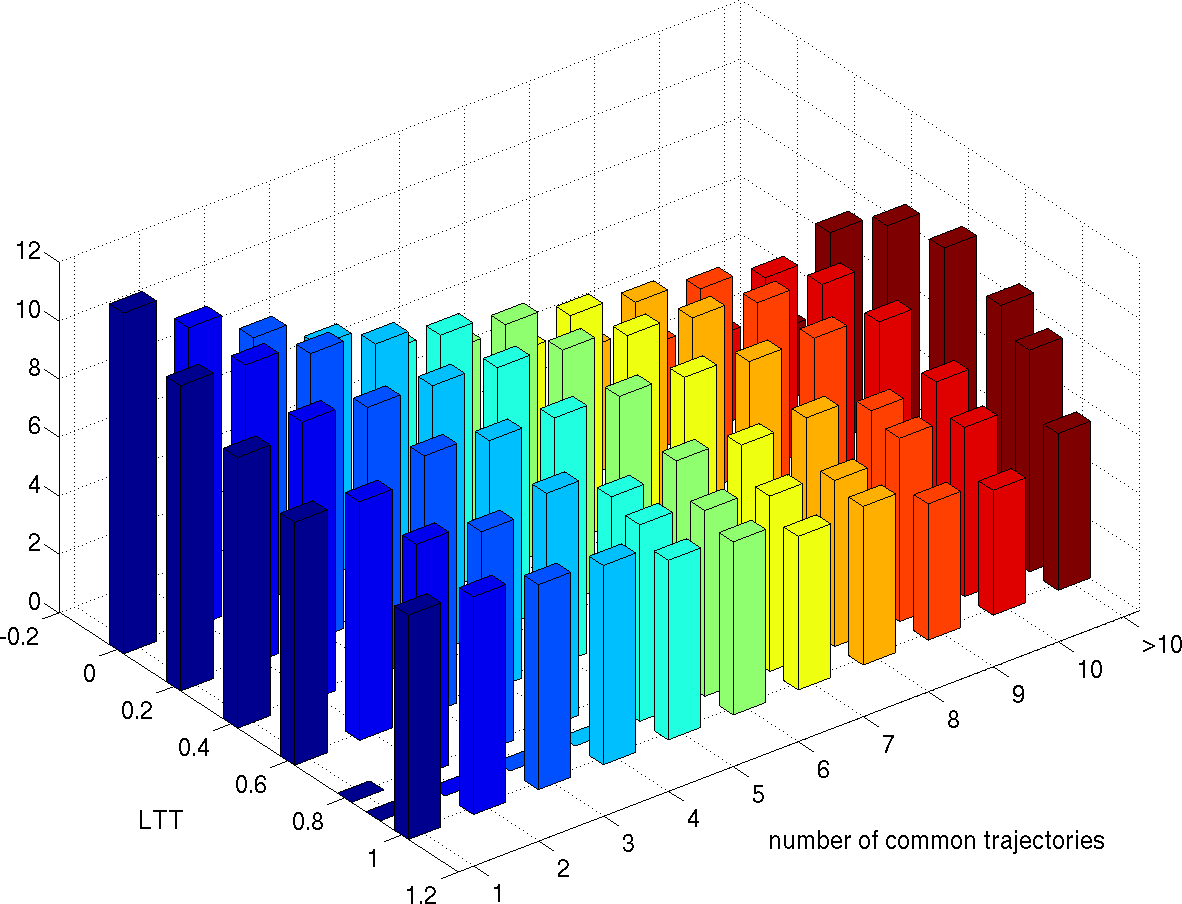
\includegraphics[width=0.47\textwidth]{images/hist/ltt_old_pos.png}}
\quad%\hfill
% \subfigure{%
% 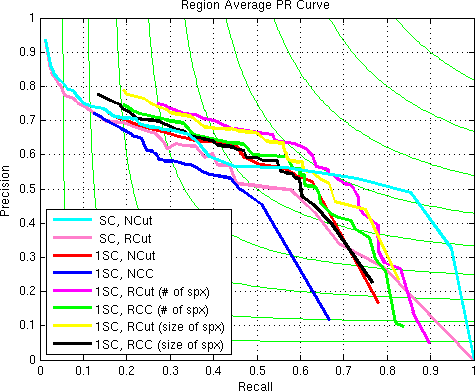
\includegraphics[trim=0cm 0cm 0cm 0.8cm, clip=true, width=0.47\textwidth]{images/basic/3.png}}
\subfigure[False Positives]{%
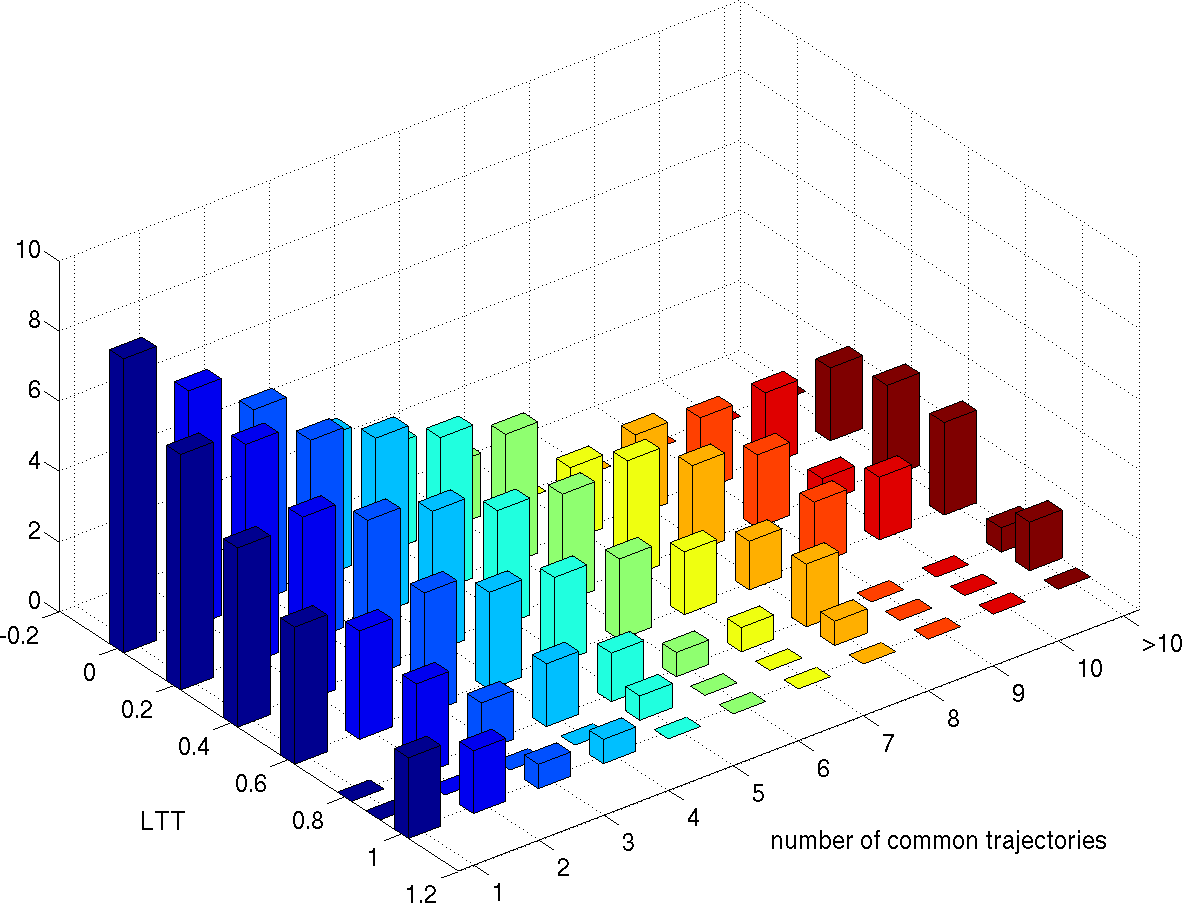
\includegraphics[width=0.47\textwidth]{images/hist/ltt_old_neg.png}}
\subfigure[Error Rate: $\mathrm{|FP|/|FP+TP|}$]{%
\centering
\scriptsize 
\renewcommand{\arraystretch}{1.3}
\begin{tabular}{|l|@{ }c@{ }|@{ }c@{ }|@{ }c@{ }|@{ }c@{ }|@{ }c@{ }|@{ }c@{ }|@{ }c@{ }|@{ }c@{ }|@{ }c@{ }|@{ }c@{ }|@{ }c@{ }|}
\hline
&\textbf{1}&\textbf{2 }&\textbf{3}&\textbf{4}&\textbf{5}&\textbf{6}&\textbf{7}&\textbf{8}&\textbf{9}&\textbf{10}&\textbf{$>$10}\\\hline
\textbf{0-0.2}&0.0363&0.0279&0.0265&0.0172&0.0196&0.0132&0&0&0&0&0\\\hline
\textbf{0.2-0.4}&0.0234&0.0177&0.0157&0.0138&0.0119&0.0106&0.0035&0.0065&0.0077&0.0123&0.0062\\\hline
\textbf{0.4-0.6}&0.0155&0.0128&0.0082&0.0059&0.0037&0.0037&0.0068&0.0037&0.0035&0.0011&0.0024\\\hline
\textbf{0.6-0.8}&0.0121&0.0062&0.0044&0.0031&0.0025&0.0023&0.0017&0.0016&0.0025&0.0033&0.0015\\\hline
\textbf{0.8-0.9}&-&0.0048&0.0021&0.0019&0.0035&0.0012&0.0016&0.0045&0&0&0.0004\\\hline
\textbf{0.9-0.99}&-&-&-&-&\textbf{0}&\textbf{0}&\textbf{0}&\textbf{0.0067}&\textbf{0}&\textbf{0}&\textbf{0.0021}\\\hline
\textbf{1}&0.0046&0.0035&0.0018&0.0022&\textbf{0}&\textbf{0}&\textbf{0}&\textbf{0}&\textbf{0}&\textbf{0}&\textbf{0}\\\hline
\end{tabular}
}
\caption[Evaluation of the LTT affinity on 4 annotated frames for each video sequence considering the number of common trajectories]{
{\bf Evaluation of the LTT affinity on 4 annotated frames for each video sequence (roughly 1st, 10th, 20th, 30th frame) considering the number of common trajectories.}}
\label{fig:ltt_10th}
\end{figure}
\subsection{Evaluation of Superpixels Affinities Between Adjacent Video Frames}
The same experiments were conducted just for the neighbouring frames.
Figure~\ref{fig:affin_adj} represents the results for all affinities, now including STT for 3 adjacent frames for each sequence. Moreover, STA and STM are also evaluated for superpixels across 1 frame apart.
The error rates for ABA and STM stay the same, but a few mistakes occur for STA. Also the drop in the performance of LTT across the adjacent frames may be observed, the error rate is more than 3\%. 
One may assume that if the number of the common trajectories is restricted like in the case above the number of errors could be decreased. 
\begin{figure}[htbp]
\centering
\addtolength{\subfigcapskip}{0.07in}
\subfigure[True Positives]{%
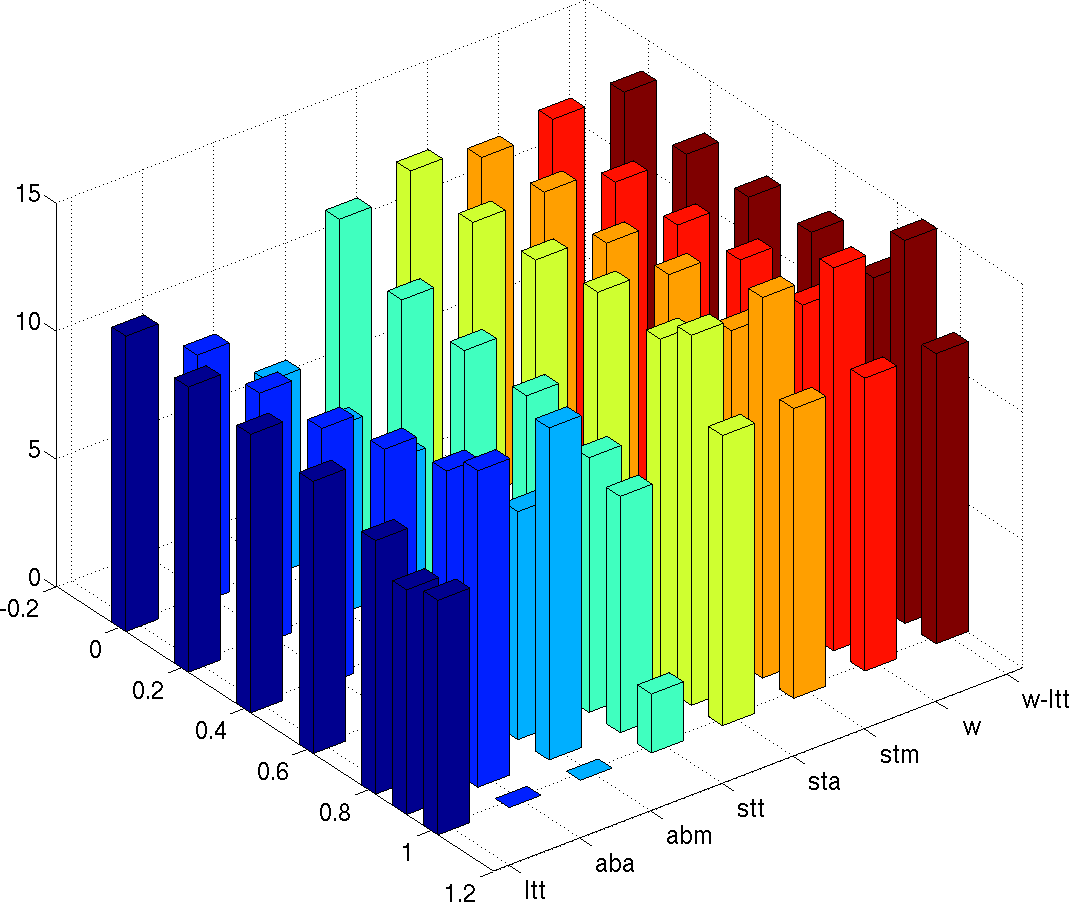
\includegraphics[width=0.45\textwidth]{images/hist/all_annot_pos.png}}
\quad%\hfill
% \subfigure{%
% 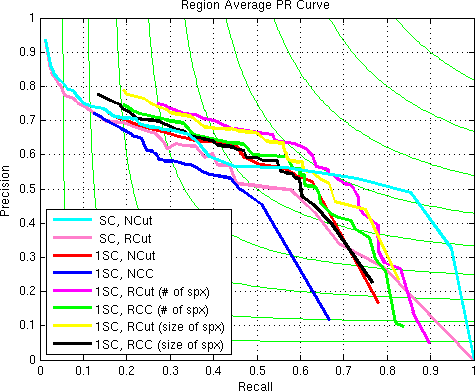
\includegraphics[trim=0cm 0cm 0cm 0.8cm, clip=true, width=0.47\textwidth]{images/basic/3.png}}
\subfigure[False Positives]{%
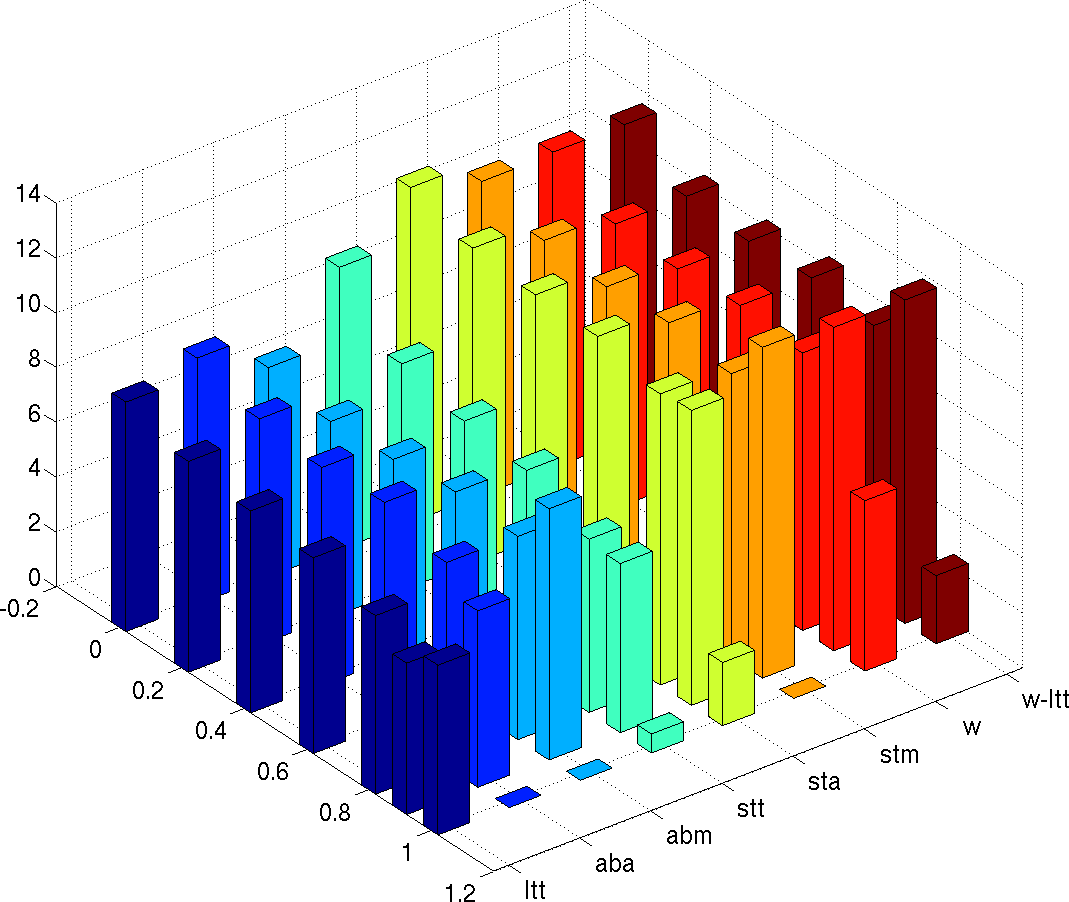
\includegraphics[width=0.45\textwidth]{images/hist/all_annot_neg.png}}
\subfigure[Error Rate: $\mathrm{|FP|/|FP+TP|}$]{%
\centering
\scriptsize 
\renewcommand{\arraystretch}{1.3}
\begin{tabular}{|l|@{ }c@{ }|@{ }c@{ }|@{ }c@{ }|@{ }c@{ }|@{ }c@{ }|@{ }c@{ }|@{ }c@{ }|@{ }c@{ }|}
\hline
&\textbf{ltt}&\textbf{aba}&\textbf{abm}&\textbf{stt}&\textbf{sta}&\textbf{stm}&\textbf{w}&\textbf{w-ltt}\\\hline
\textbf{0-0.2}&0.0402&0.3198&0.4978&0.0683&0.1797&0.1476&0.1085&0.1095\\\hline
\textbf{0.2-0.4}&0.0307&0.1696&0.4434&0.0437&0.1386&0.0658&0.0852&0.0843\\\hline
\textbf{0.4-0.6}&0.0289&0.1099&0.3809&0.0356&0.1035&0.0789&0.0801&0.0793\\\hline
\textbf{0.6-0.8}&0.0295&0.0655&0.2961&0.0312&0.0741&0.0662&0.0748&0.0745\\\hline
\textbf{0.8-0.9}&0.0325&0.0163&0.1834&0.0258&0.0524&0.0817&0.0701&0.0698\\\hline
\textbf{0.9-0.99}&0.0371&\textbf{0.0026}&0.0216&0.0446&0.0241&0.0569&0.0405&0.0405\\\hline
\textbf{1}&0.0485&-&-&0.1667&\textbf{0.0001}&\textbf{0}&0.0053&0.0001\\\hline
\end{tabular}
}
\caption[Evaluation of the LTT, ABA, ABM, STT, STA, STM, W, W-LTT affinities on 3 adjacent annotated frames for each video sequence]{
{\bf Evaluation of the LTT, ABA, ABM, STT, STA, STM, W, W-LTT affinities on 3 adjacent annotated frames for each video sequence.}}
\label{fig:affin_adj}
\end{figure}

%The LTT affinity performs worse across 1 or 2 frames and it could be assumed that the overall performance of the algorithm may be boosted if we consider it only between superpixels of the non-adjacent frames.
\begin{figure}[htbp]
\centering
\addtolength{\subfigcapskip}{0.07in}
\subfigure[True Positives]{%
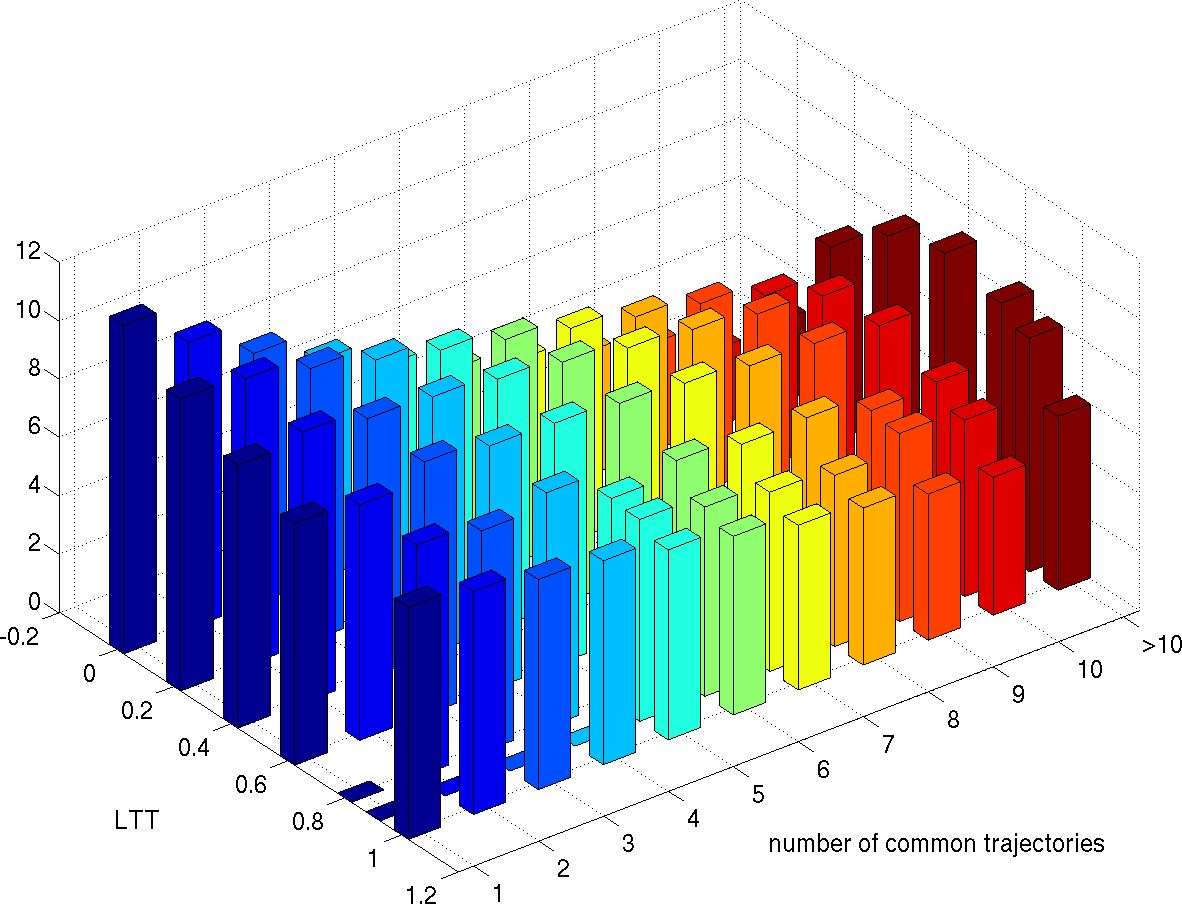
\includegraphics[width=0.47\textwidth]{images/hist/ltt_annot_pos.png}}
\quad
\subfigure[False Positives]{%
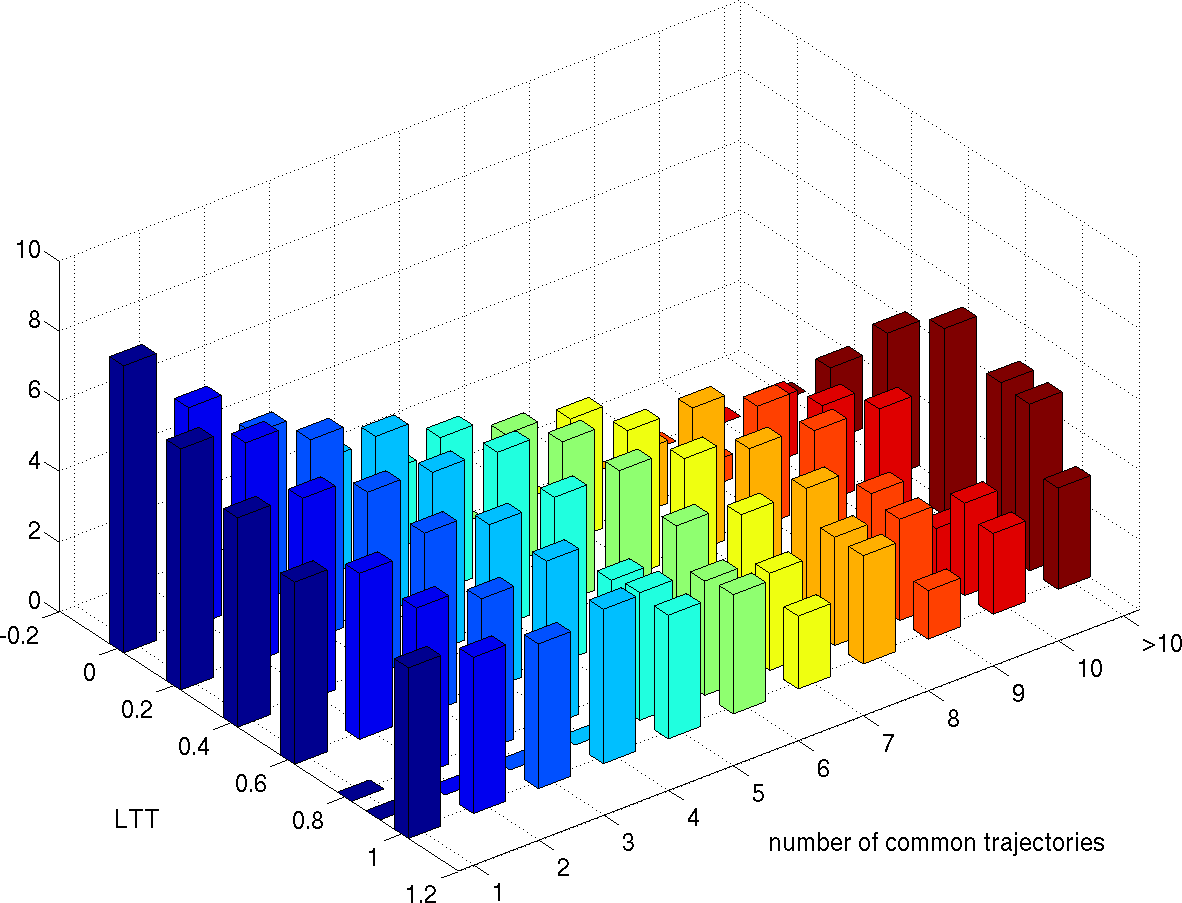
\includegraphics[width=0.47\textwidth]{images/hist/ltt_annot_neg.png}}
\subfigure[Error Rate: $\mathrm{|FP|/|FP+TP|}$]{%
\centering
\scriptsize 
\renewcommand{\arraystretch}{1.3}
\begin{tabular}{|l|@{ }c@{ }|@{ }c@{ }|@{ }c@{ }|@{ }c@{ }|@{ }c@{ }|@{ }c@{ }|@{ }c@{ }|@{ }c@{ }|@{ }c@{ }|@{ }c@{ }|@{ }c@{ }|}
\hline
&\textbf{1}&\textbf{2 }&\textbf{3}&\textbf{4}&\textbf{5}&\textbf{6}&\textbf{7}&\textbf{8}&\textbf{9}&\textbf{10}&\textbf{$>$10}\\\hline
\textbf{0-0.2}&0.0451&0.0285&0.0233&0.0156&0.0158&0&0&0&0&0&0\\\hline
\textbf{0.2-0.4}&0.0419&0.0295&0.0263&0.0249&0.0199&0.0175&0.0213&0.0065&0.0032&0.0167&0.0101\\\hline
\textbf{0.4-0.6}&0.0461&0.0303&0.0264&0.0256&0.0285&0.0247&0.0241&0.0281&0.0202&0.0129&0.0151\\\hline
\textbf{0.6-0.8}&0.0436&0.0347&0.0291&0.0249&0.0287&0.0356&0.0294&0.0248&0.0223&0.0257&0.0247\\\hline
\textbf{0.8-0.9}&-&0.0412&0.0379&0.0349&0.0286&0.0418&0.0383&0.0377&0.0293&0.0048&0.0236\\\hline
\textbf{0.9-0.99}&-&-&-&-&0.0366&0.0384&0.0335&0.0591&0.0279&0.0321&0.0374\\\hline
\textbf{1}&0.0444&0.0399&0.0445&0.0708&0.0486&0.0625&0.0278&0.0924&0.0263&0.0819&0.0448\\\hline
\end{tabular}
}
\caption[Evaluation of the LTT affinity on 3 adjacent annotated frames for each video sequence considering the number of common trajectories]{
{\bf Evaluation of the LTT affinity on 3 adjacent annotated frames for each video sequence considering the number of common trajectories.}}
\label{fig:ltt_adj}
\end{figure}

Figure~\ref{fig:ltt_adj} shows the detailed evaluation of LTT across neighbouring frames.
As it can be observed the error rate does not decrease with increasing number of trajectories. 
For the LTT it is easier to achieve higher values between superpixels in the adjacent frames and with a fewer intersecting point trajectories and therefore it is less reliable for those particular cases. 

The majority of the errors could be avoided if the LTT is not considered for the superpixels in the neighbouring frames and only takes into account superpixels with the number of common trajectories higher or equal 5.
Following this recommendation the overall performance of the algorithm could be improved.
\section{Discussion}
\label{ch3:disc}
From the presented above experiments we saw a good performance of low-level features. It was observed that the error rate is quite low for the affinities which achieve high score values. 
The features were gained by integrating local grouping cues and calculated by using different types of information: appearance as well as motion and spatial overlap of superpixels.
%The proposed terms allowed to calculate within- and between-frame affinities, that could be across a potentially large number of frames due to the long-term nature of point trajectories.
However, to produce high-quality results video segmentation should not only consider local cue models, but also allow more global reasoning of appearance and motion.

It was also observed that some similarity measures were overlooked by the previous method of~\cite{GalassoCS12} and might be outweighed by the other affinities in the final score.
A way to deal with this problem would be to learn the final score of the affinity matrix from raw features or low-level features of the video. However, the main difficulty
of this approach is the lack of directly defined objective function that could well represent an impact of learned affinities on the produced clustering results and benchmark metrics.